
In this chapter, we present the evaluation results for JOP. In the
following section, the hardware platform that is used for
benchmarking is described. This is followed by a comparison of JOP's
resource usage with other soft-core processors. In
Section~\ref{sec:performance} the performance of a number of
different solutions for embedded Java is compared with embedded
application benchmarks. Comparison at bytecode level can be found in
\cite{jop:austrochip05}. This chapter concludes with a description of
real-world applications based on JOP.

\section{Hardware Platforms}

During the development of JOP and its predecessors, several
different FPGA boards were developed. The first experiments involved
using Altera FPGAs EPF8282,\linebreak[4] EPF8452, EPF10K10 and ACEX
1K30 on boards that were connected to the printer port of a PC for
configuration, download and communication. The next step was the
development of a stand-alone board with FLASH memory and static RAM.
This board was developed in two variants, one with an ACEX 1K50 and
the other with a Cyclone EP1C6 or EP1C12. Both boards are
pin-compatible and are used in commercial applications of JOP. The
Cyclone board is the hardware that is used for the following
evaluations.

This board is an ideal development platform for JOP. Static RAM and
FLASH are connected via independent buses to the FPGA. All unused
FPGA pins and the serial line are available via four connectors. The
FLASH can be used to store configuration data for the FPGA and
application program/data. The FPGA can be configured with a
ByteBlasterMV download cable or loaded from the FLASH (with a small
CPLD on board). As the FLASH is also connected to the FPGA, it can be
programmed from the FPGA. This allows for upgrades of the Java
program and even the processor core itself in the field. The board is
slightly different from other FPGA prototyping boards, in that its
connectors are on the bottom side. Therefore, it can be used as a
module (60~mm x 48~mm), i.e.\ as part of a larger board that contains
the periphery. The Cyclone board contains:
%
%\begin{samepage}
\begin{itemize}
\item Altera Cyclone EP1C6Q240 or EP1C12Q240
\item Step Down voltage regulator (1V5)
\item Crystal clock (20~MHz) at the PLL input (up to 640~MHz
    internal)
\item 512~KB FLASH (for FPGA configuration and program code)
\item 1~MB fast asynchronous RAM (15 ns)
\item Up to 128~MB NAND FLASH
\item ByteBlasterMV port
\item Watchdog with a LED
\item EPM7064 PLD to configure the FPGA from the FLASH on watchdog reset
\item Serial interface driver (MAX3232)
\item 56 general-purpose IO pins
\end{itemize}
%\end{samepage}
%
The RAM consists of two independent 16-bit banks (with their own
address and control lines). Both RAM chips are on the bottom side of
the PCB, directly under the FPGA pins. As the traces are very short
(under 10~mm), it is possible to use the RAMs at full speed without
reflection problems. The two banks can be combined to form 32-bit
RAM or support two independent CPU cores. Pictures and the schematic
of the board can be found in Appendix~\ref{appx:cycore}.

\index{Baseio}

The expansion board Baseio hosts the CPU module and provides a
complete Java processor system with Internet connection. A step down
switching regulator with a large AC/DC input range supplies the core
board. All input and output pins are EMC/ESD-protected and routed to
large connectors (5.08~mm Phoenix). Analog comparators can be used to
build sigma-delta ADCs. For FPGA projects with a network connection,
a CS8900 Ethernet controller with an RJ45 connector is included on
the expansion board. Pictures and the schematic of the board can be
found in Appendix~\ref{appx:baseio}.


\section{Chip Area and Clock Frequency}

Cost is an important issue for embedded systems. The cost of a chip
is directly related to the die size (the cost per die is roughly
proportional to the square of the die area \cite{Hennessy02}).
Processors for embedded systems are therefore optimized for minimum
chip size. In this section, we will compare JOP with different
processors in terms of size. One major design objective in the
development of JOP was to create a small system that can be
implemented in a low-cost FPGA.


Table~\ref{tab:soft-cores} compares the resource consumption and
maximum clock frequency of a time-predictable processor (JOP), a
standard MIPS architecture (YARI), the LEON SPARC processor, and a
complex Java processor (picoJava), when implemented in the same FPGA
(Altera EP1C6/12 FPGA \cite{AltCyc}). For the resource comparison we
compare the consumption of the two basic structures of an FPGA; Logic
Cells (LC) and embedded memory blocks. The maximum frequency for all
soft-core processors is in the same technology.

\begin{table}
  \begin{center}
    \begin{tabular}[t]{lrrr}
        \toprule
      Soft-core    & Logic Cells & Memory  & Frequency \\
        \midrule
      JOP          & 3,300       &  7.6 KB & 100~MHz    \\
      YARI         & 6,668       & 18.9 KB & 75~MHz     \\
      LEON3        & 7,978       & 10.9 KB & 35~MHz \\
      picoJava     & 27,560      & 47.6 KB & 40~MHz     \\
        \bottomrule
    \end{tabular}
  \end{center}
    \caption{Resource consumption and maximum operating frequency of JOP, YARI, LEON3, and picoJava.}
    \label{tab:soft-cores}
\end{table}

%        Lightfoot\footnotemark \cite{Lightfoot} & 3400 & 4 & 40 \\
%        NIOS A \cite{NIOS} & 1828 & 6.2 & 120 \\
%        NIOS B \cite{NIOS} & 2923 & 5.5 & 119 \\
%        SPEAR\footnotemark \cite{Delvai:ECRTS2003} & 1700 & 8 & 80 \\

JOP is configured with a 1~KB stack cache, 2~KB microcode ROM, and
4~KB method cache with 16 blocks. YARI is a MIPS compatible soft-core
\cite{cacao:yari:techrep}, optimized for FPGA technology. YARI is
configured with a 4-way set-associative instruction cache and a 4-way
set-associative write-through data cache. Both caches are 8~KB. LEON3
\cite{LEON}, the open-source implementation of the SPARC V8
architecture, has been ported to the exact same hardware that was
used for the JOP numbers. LEON3 is representative for a RISC
processor that is used in embedded real-time systems (e.g., by ESA
for space missions). The size a frequency numbers of picoJava-II
\cite{pJ1} are taken from an implementation in a Altera Cyclone-II
FPGA \cite{master:puffitsch}.



The streamlined architecture of JOP results in a small design: JOP is
half the size of the MIPS core YARI or the SPARC core LEON. Compared
with picoJava JOP consumes about 12\% of the resources. JOP's size
allows implementing a CMP version of JOP even in a low-cost FPGA. The
simple pipeline of JOP achieves the highest clock frequency of the
three designs. From the frequency comparison we can estimate that the
maximum clock frequency of JOP in an ASIC will also be higher than a
standard RISC pipeline in an ASIC.

%The vendor independent and open-source RISC processor LEON can be
%clocked only with 35\% of JOP's frequency.

To prove that the VHDL code for JOP is as portable as possible, JOP
was also implemented in a Xilinx Spartan-3 FPGA \cite{Spartan3}. Only
the instantiation and initialization code for the on-chip memories is
vendor-specific, whilst the rest of the VHDL code can be shared for
the different targets. JOP consumes about the same LC count in the
Spartan device, but has a slower clock frequency (83~MHz).


%All configurations of JOP contain the on-chip microcode memory, the
%1~KB stack cache, a 1~KB method cache, a memory interface to a
%32-bit static RAM, and an 8-bit FLASH interface for the Java program
%and the FPGA configuration data. The minimum configuration
%implements multiplication and the shift operations in microcode. In
%the typical configuration, these operations are implemented as a
%sequential Booth multiplier and a single-cycle barrel shifter. The
%typical configuration also contains some useful I/O devices such as
%an UART and a timer with interrupt logic for multi-threading. The
%typical configuration of JOP consumes about 30\% of the LCs in a
%Cyclone EP1C6, thus leaving enough resources free for
%application-specific logic.

%As a reference, NIOS \cite{NIOS}, Altera's popular RISC soft-core, is
%also included in \tablename~\ref{tab_results_compare}. NIOS has a
%16-bit instruction set, a 5-stage pipeline and can be configured with
%a 16 or 32-bit datapath. Version A is the minimum configuration of
%NIOS. Version B adds an external memory interface, multiplication
%support, and a timer. Version A is comparable with the minimal
%configuration of JOP, and Version B with its typical configuration.



Table~\ref{tab:results:gate:count} provides gate count estimates for
JOP, picoJava, the aJile processor, and, as a reference, an old Intel
Pentium MMX processor. Equivalent gate count for an LC\footnote{The
factors are derived from the data provided for various processors in
Chapter~\ref{chap:related} and from the resource estimates in
\cite{jop:stack}.} varies between 5.5 and 7.4 -- we chose a factor of
6 gates per LC and 1.5 gates per memory bit for the estimated gate
count for JOP in the table. JOP is listed in the typical
configuration that consumes 3300 LCs. The Pentium MMX contains 4.5M
transistors \cite{pentium:mmx} that are equivalent to 1125K gates.

%Different LC/gate values:
%    from tow-level stack: 1LC = 5.4 gates
%    from ram stack: 1LC = 5.5 gates
%    from register stack: 1LC = 5.9 gates
%    Moon: 3660LCs - 27K gates + 3KB ROM + 1KB RAM: 1LC = 7.4 gates
%    Lightfoot: 3400LCs - 25K gates: 1LC = 7.4 gates
%    picoJava: ROM/RAM - 1Bit = 1 gate
%
%    JOP: 1831 LCs, 3.25KB: 1831*6 + 26624*1.5 = 11K + 39k
%    JOP: 2050*6 + 3.5*1024*8*1.5 = 12K + 43K
%    JOP: 3300*6 + 7.6*1024*8*1.5 = 20K + 93K
%    Pentium MMX: 4.5 Mio. Transistors -> 1100K

\begin{table}
    \centering
    \begin{tabular}{lrrr}
        \toprule
        Processor & \multicolumn{1}{c}{Core} & \multicolumn{1}{c}{Memory} & \multicolumn{1}{c}{Sum.} \\
        & \multicolumn{1}{c}{(gate)} & \multicolumn{1}{c}{(gate)} & \multicolumn{1}{c}{(gate)}\\
        \midrule
        JOP & 20K & 93K & 113K\\
        picoJava & 128K & 314K & 442K\\
        aJile & 25K & 912K & 937K\\
        Pentium MMX & & & 1125K\\
        \bottomrule
    \end{tabular}
    \caption{Gate count estimates for various processors}
    \label{tab:results:gate:count}
\end{table}

We can see from the table that the on-chip memory dominates the
overall gate count of JOP, and to an even greater extent, of the
aJile processor. The aJile processor is roughly the same size as the
Pentium MMX, and both are about 10 times larger than JOP.


\section{Performance} \label{sec:performance}

One important question remains: is a time-predictable processor slow?
We evaluate the average case performance of JOP by comparing it with
other embedded Java systems: Java processors from industry and
academia and two just-in-time (JIT) compiler based systems. For the
comparison we use \code{JavaBenchEmbedded},\footnote{Available at
\url{http://www.jopwiki.com/JavaBenchEmbedded}.} a set of open-source
Java benchmarks for embedded systems. \code{Kfl} and \code{Lift} are
two real-world applications adapted with a simulation of the
environment to run as stand-alone benchmarks. \code{UdpIp} is a
simple client/server test program that uses a TCP/IP stack written in
Java.

\begin{table}
    \centering
    \begin{tabular}{lD{.}{.}{2}D{.}{.}{2}D{.}{.}{2}}
        \toprule

 & \multicolumn{1}{c}{Kfl}
    & \multicolumn{1}{c}{UdpIp} & \multicolumn{1}{c}{Lift}\\
        \midrule
Cjip & 176 & 91 & \\
jamuth & 3400 & 1500 & \\
EJC & 9893 &  2882 & \\
SHAP & 11570 & 5764 & 12226 \\
aJ100 & 14148 & 6415 & \\
JOP & 19907 & 8837 & 18930 \\
picoJava & 23813 & 11950 & 25444 \\
CACAO/YARI & 39742 & 17702 & 38437 \\
        \bottomrule
    \end{tabular}
    \caption{Application benchmark performance on different Java systems.
    The table shows the benchmark results in
    iterations per second -- a higher
    value means higher performance.
    }
    \label{tab:results}
\end{table}


Table~\ref{tab:results} shows the raw data of the performance
measurements of different embedded Java systems for the three
benchmarks. The numbers are iterations per second whereby a higher
value represents better performance. Figure~\ref{fig:bench} shows the
results scaled to the performance of JOP.

The numbers for JOP are taken from an implementation in the Altera
Cyclone FPGA \cite{AltCyc}, running at 100~MHz. JOP is configured
with a 4~KB method cache and a 1~KB stack cache.

\begin{figure}[t]
    \centering
    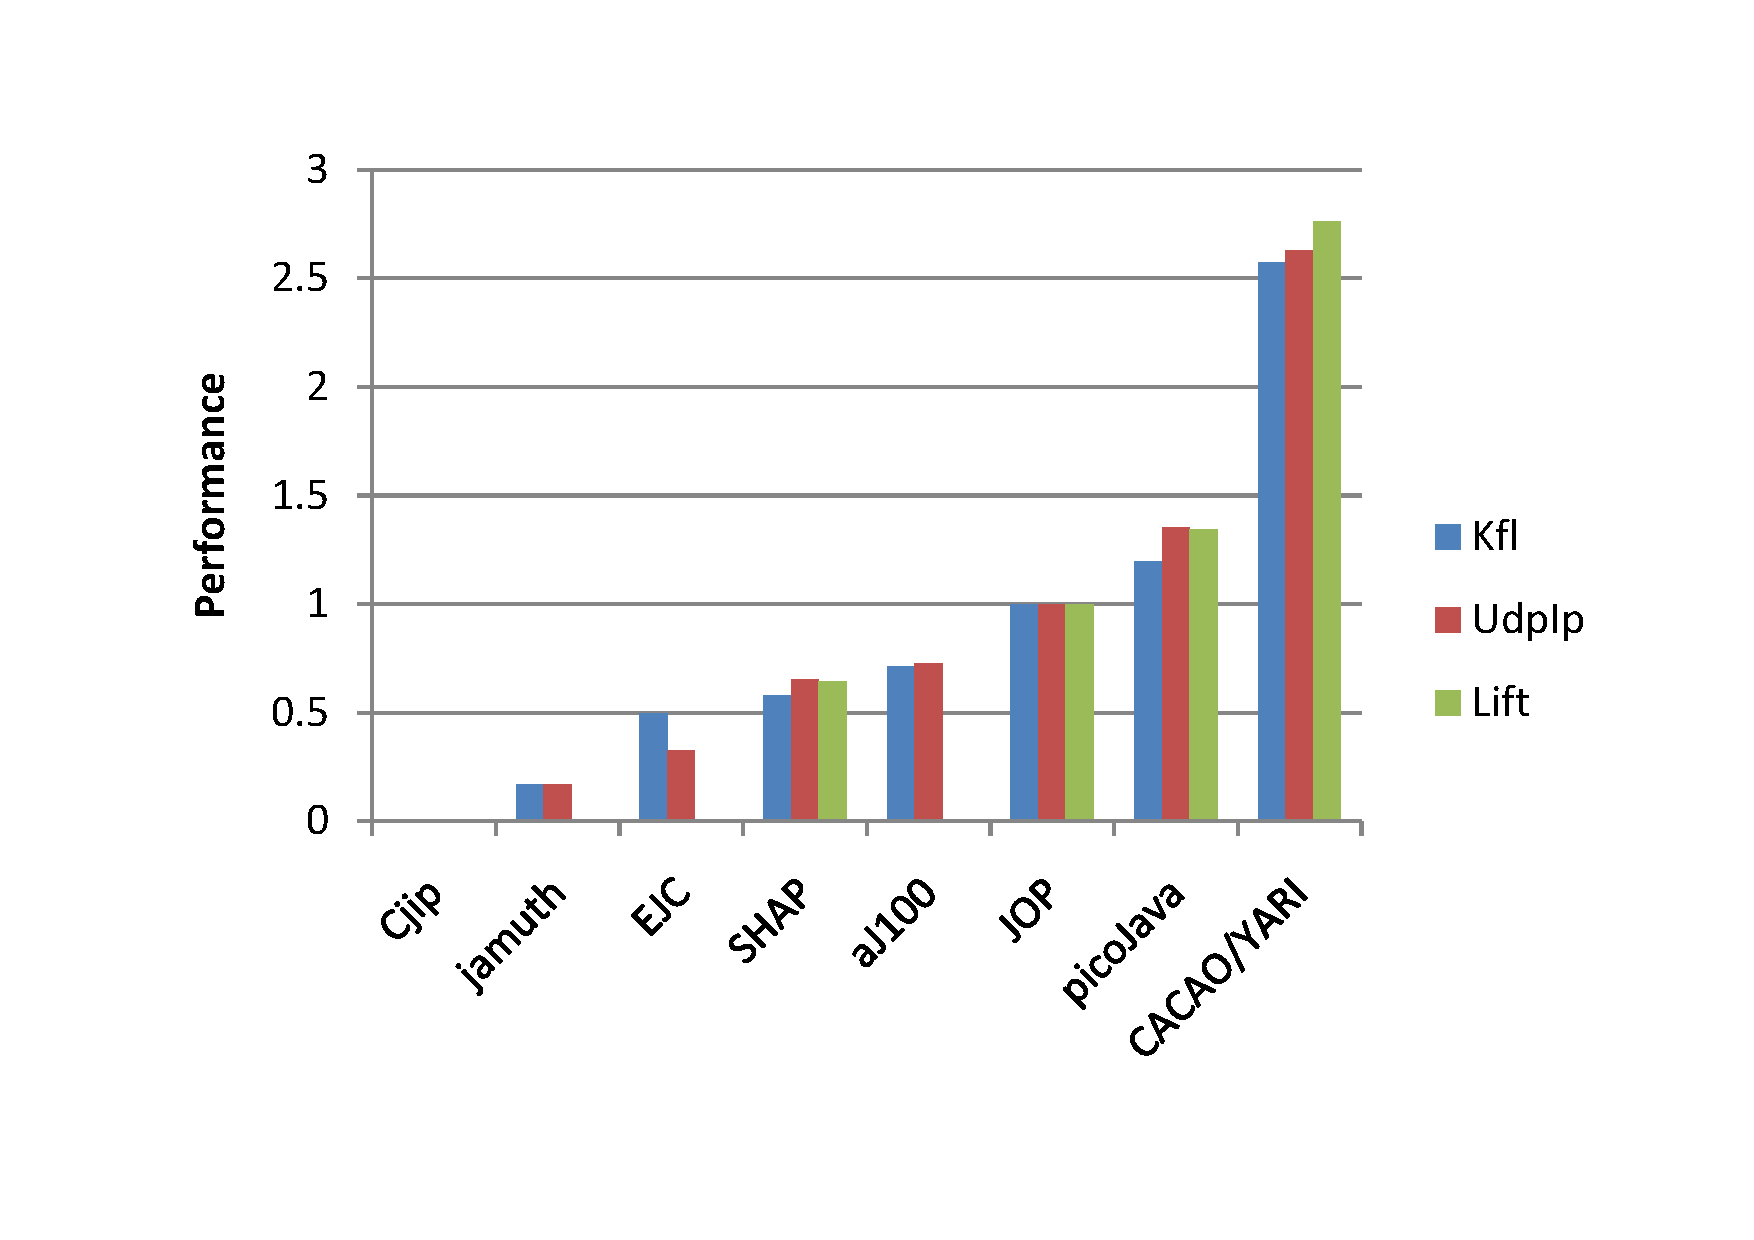
\includegraphics[width=\excelwidth]{results/perf}
    \caption{Performance comparison of different Java systems with
    embedded application benchmarks. The results are scaled to the performance of JOP}
    \label{fig:bench}
\end{figure}

Cjip \cite{Cjip} and aJ100 \cite{aJile} are commercial Java
processors, which are implemented in an ASIC and clocked at 80 and
100~Mhz, respectively. Both cores do not cache instructions. The
aj100 contains a 32~KB on-chip stack memory. jamuth
\cite{jamuth:jtres07} and SHAP \cite{shap} are Java processors that
are implemented in an FPGA. jamuth is the commercial version of the
Java processor Komodo \cite{komodo2003}, a research project for
real-time chip multithreading. jamuth is configured with a 4~KB
direct-mapped instruction cache for the measurements. The
architecture of SHAP is based on JOP and enhanced with a hardware
object manager. SHAP also implements the method cache
\cite{shap:mcache}. The benchmark results for SHAP are taken from the
SHAP website.\footnote{\url{http://shap.inf.tu-dresden.de/}, accessed
December, 2008} SHAP is configured with a 2~KB method cache and 2~KB
stack cache.

picoJava \cite{pJ1} is a Java processor developed by Sun. picoJava is
no longer produced and the second version (picoJava-II) was available
as open-source Verilog code. Puffitsch implemented picoJava-II in an
FPGA (Altera Cyclone-II) and the performance numbers are obtained
from that implementation \cite{master:puffitsch}. picoJava is
configured with a direct-mapped instruction cache and a 2-way
set-associative data cache. Both caches are 16~KB.

EJC \cite{EJC} is an example of a JIT system on a RISC processor
(32-bit ARM720T at 74~MHz). The ARM720T contains an 8~KB unified
cache. To compare JOP with a JIT based system in exactly the same
hardware we use the research JVM CACAO \cite{cacao} on top of the
MIPS compatible soft-core YARI \cite{cacao:yari}. YARI is configured
with a 4-way set-associative instruction cache and a 4-way
set-associative write-through data cache. Both caches are 8~KB.

The measurements do not provide a clear answer to the question of
whether a time-predictable architecture is slow. JOP is about 40\%
faster than the commercial Java processor aJ100, but picoJava is 30\%
faster than JOP and the JIT/RISC combination (CACAO/YARI) is about
2.7 times faster than JOP. We conclude that a time-predictable
solution will never be as fast in the average case as a solution
optimized for the average case.

%%\subsection{Notes for targets}
%%
%%\subsubsection{JStamp}
%%
%%\begin{verbatim}
%%    aJile project in \usr2\ajile\bench
%%    Sources from JOP target
%%    LowLevel.java from directory aJile
%%    Remove .class in ...\dist\classes
%%    Generate .class with \bat\ajc.bat in source directory
%%        destination is ...\dist\classes
%%        e.g. in ...\src\bench: ajc jbe/DoAll
%%    aJile ChemBuilder (bench.ajp) use COM1 for System.out
%%    Terminal on Serial A, 9600 baud
%%        Did not get the System.out in Charade (but it worked some
%%        time ago)
%%    Charade: Reset, File-Load \usr2\ajile\bench\build.bin
%%\end{verbatim}


\section{Applications}
\label{sec:applications}

During the research for the PhD thesis, the first working version of
JOP was used in a real-world application. Using an architecture under
development in a commercial project entails risks. Nevertheless, this
was deemed to be the best way to prove the feasibility of the
processor. In this section, the experiences of the first project
involving JOP are summarized.

\subsection{Motor Control}
\label{sec:app:kfl}

In rail cargo, a large amount of time is spent on loading and
unloading of goods wagons. The contact wire above the wagons is the
main obstacle. Balfour Beatty Austria developed and patented a
technical solution, the so-called \emph{Kippfahrleitung}, to tilt up
the contact wire. This is done on a line up to one kilometer. An
asynchronous motor on each mast is used for this tilting. However, it
has to be done synchronously on the whole line.

Each motor is controlled by an embedded system. This system also
measures the position and communicates with a base station.
\figurename~\ref{fig:results:kfl:mast} shows the mast with the motor
and the control system in the `down' and `up' positions. The base
station has to control the deviation of individual positions during
the tilt. It also includes the user interface for the operator. In
technical terms, this is a distributed, embedded real-time control
system, communicating over an RS485 network.

\begin{figure}
    \centering
    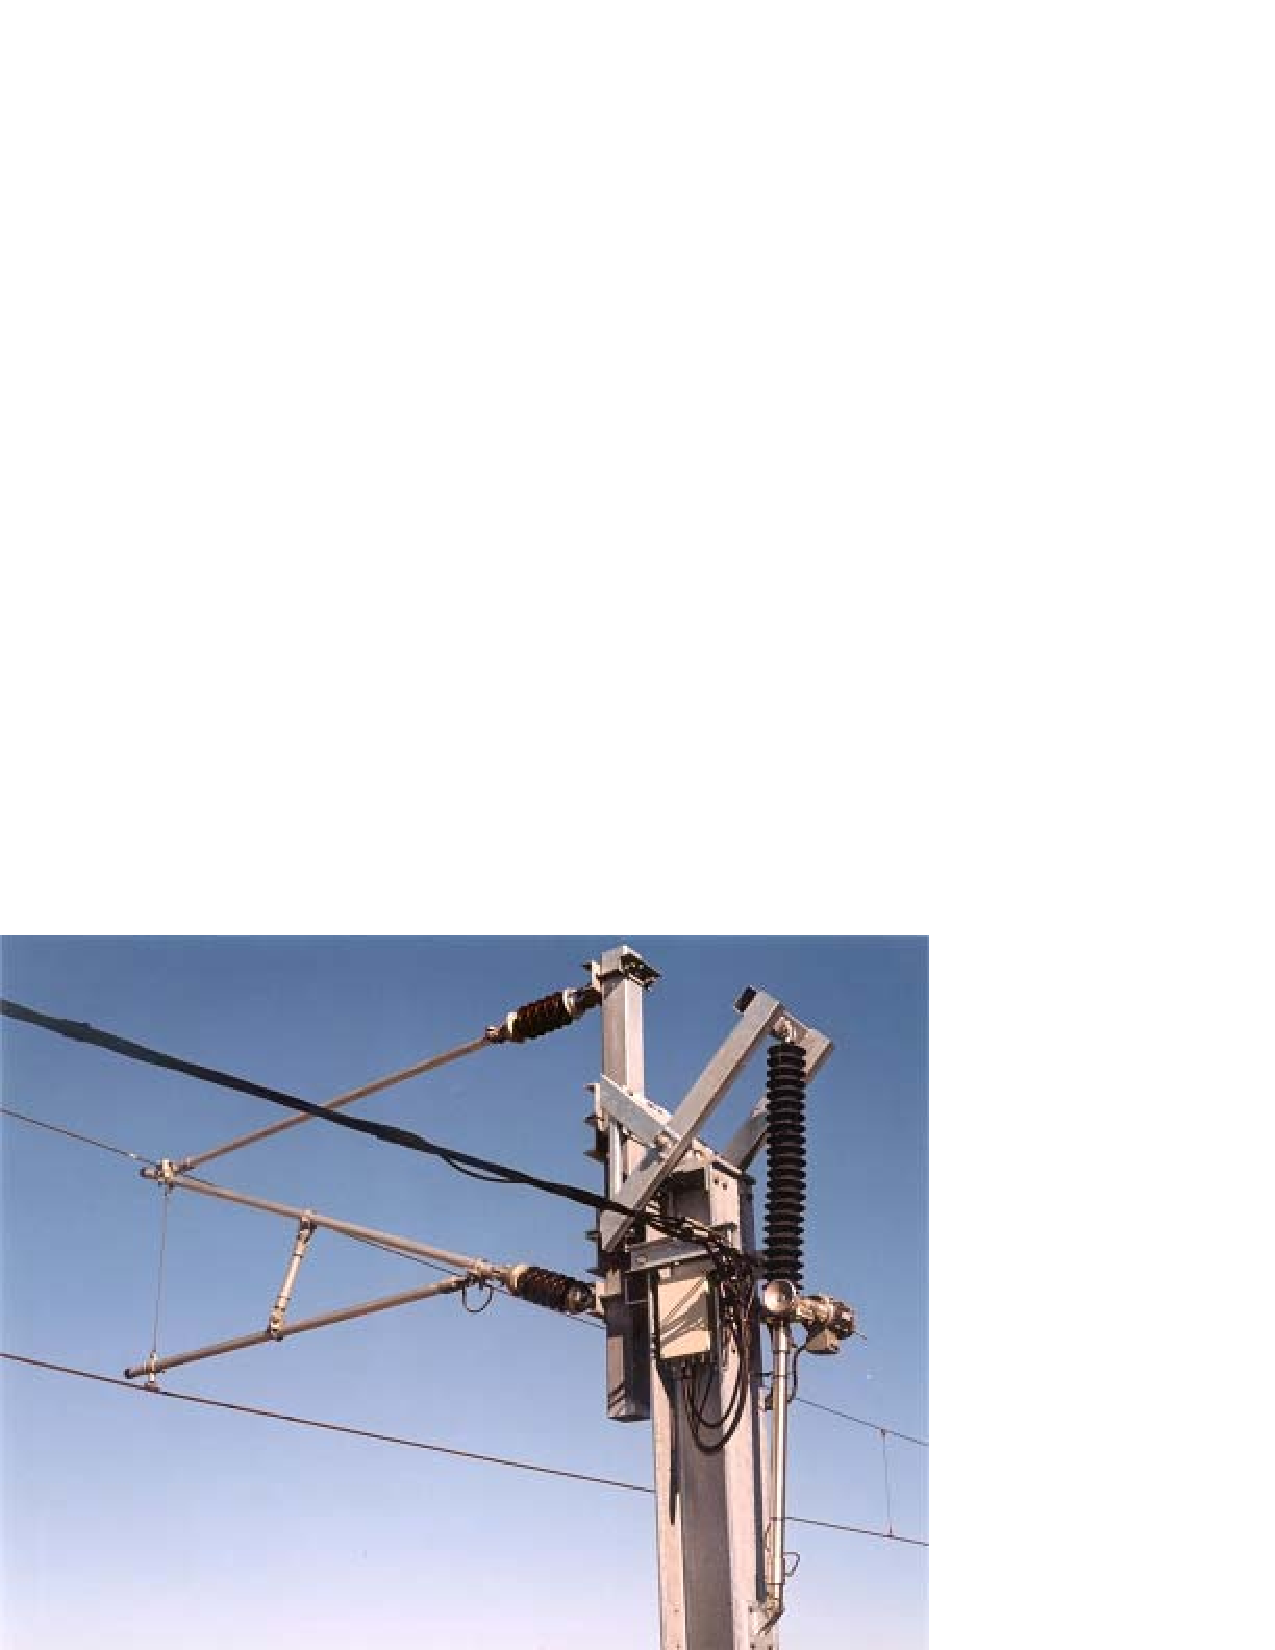
\includegraphics[width=7cm]{results/results_kfl_mast1}
    \hspace{1cm}
    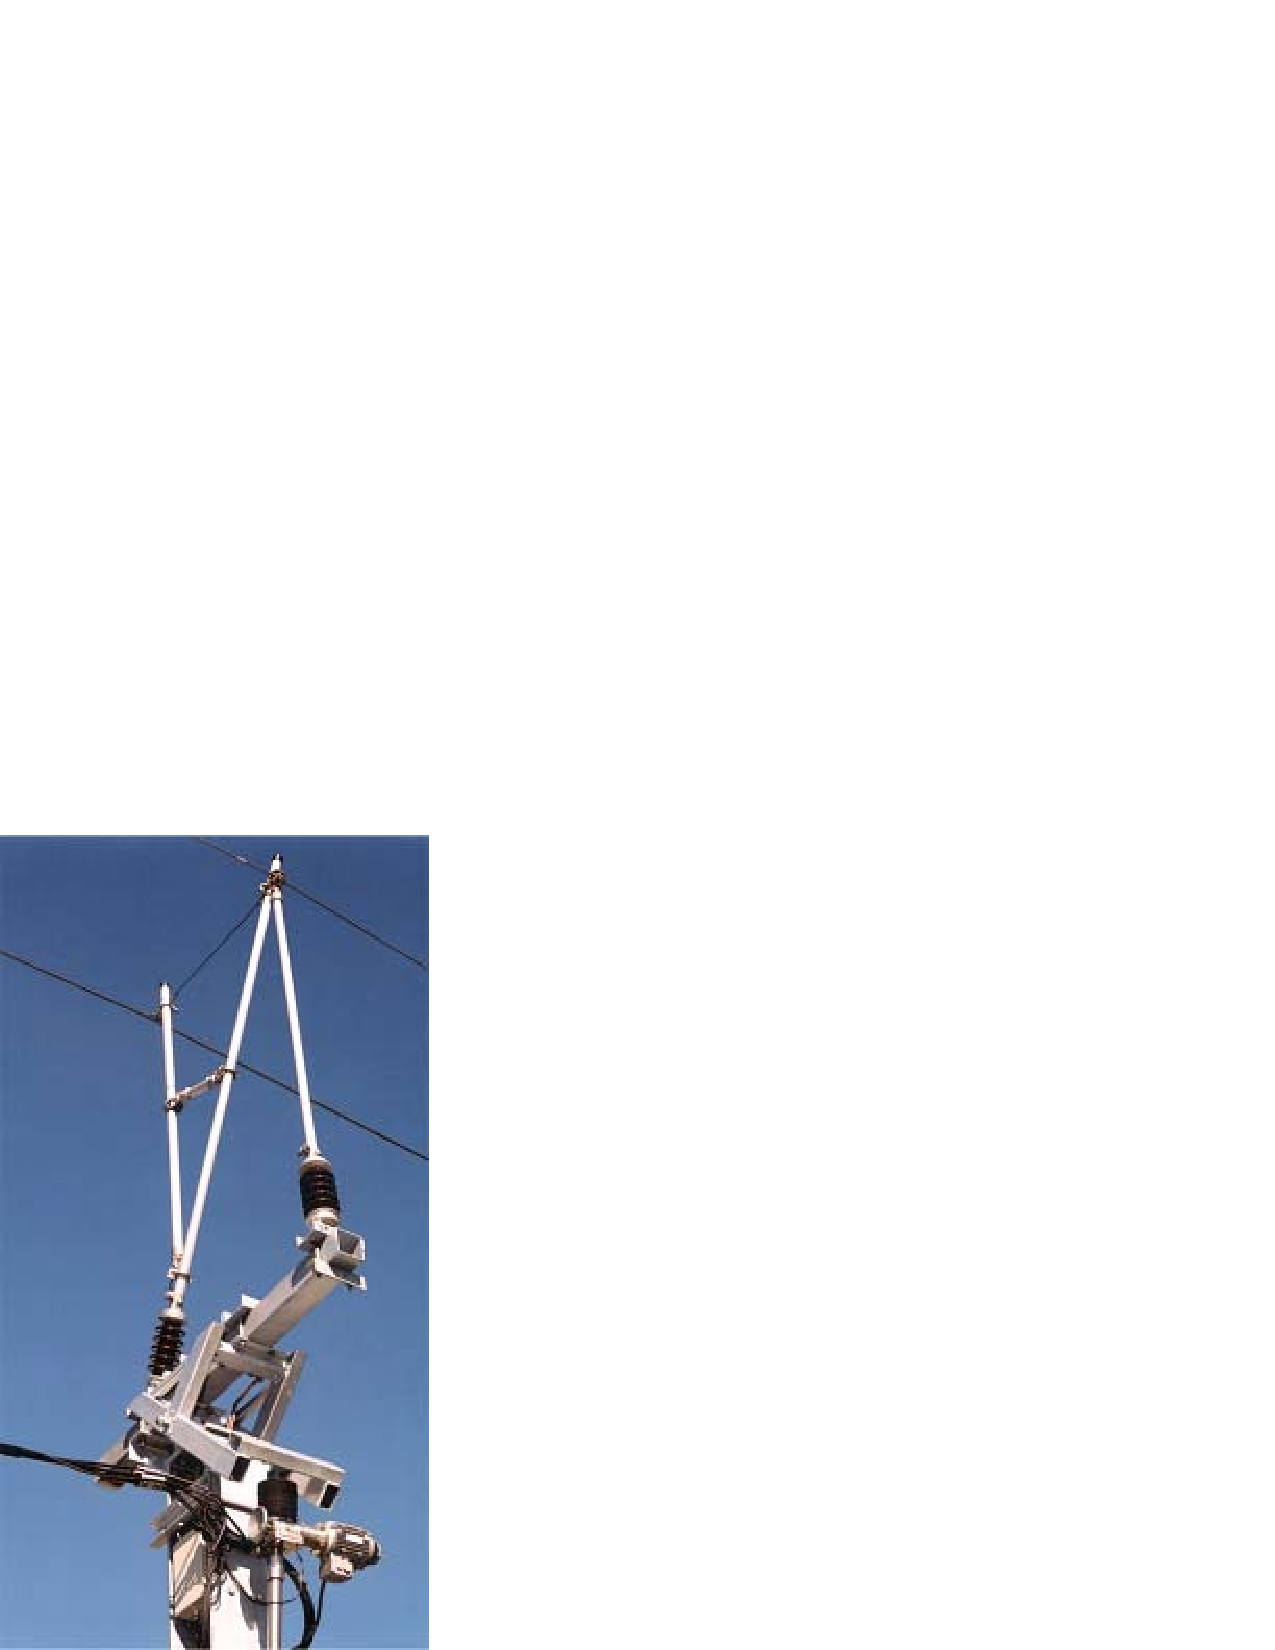
\includegraphics[width=4cm]{results/results_kfl_mast2}
    \caption{Picture of a \emph{Kippfahrleitung} mast in down and up position}
    \label{fig:results:kfl:mast}
\end{figure}

%\begin{figure}
%    \centering
%    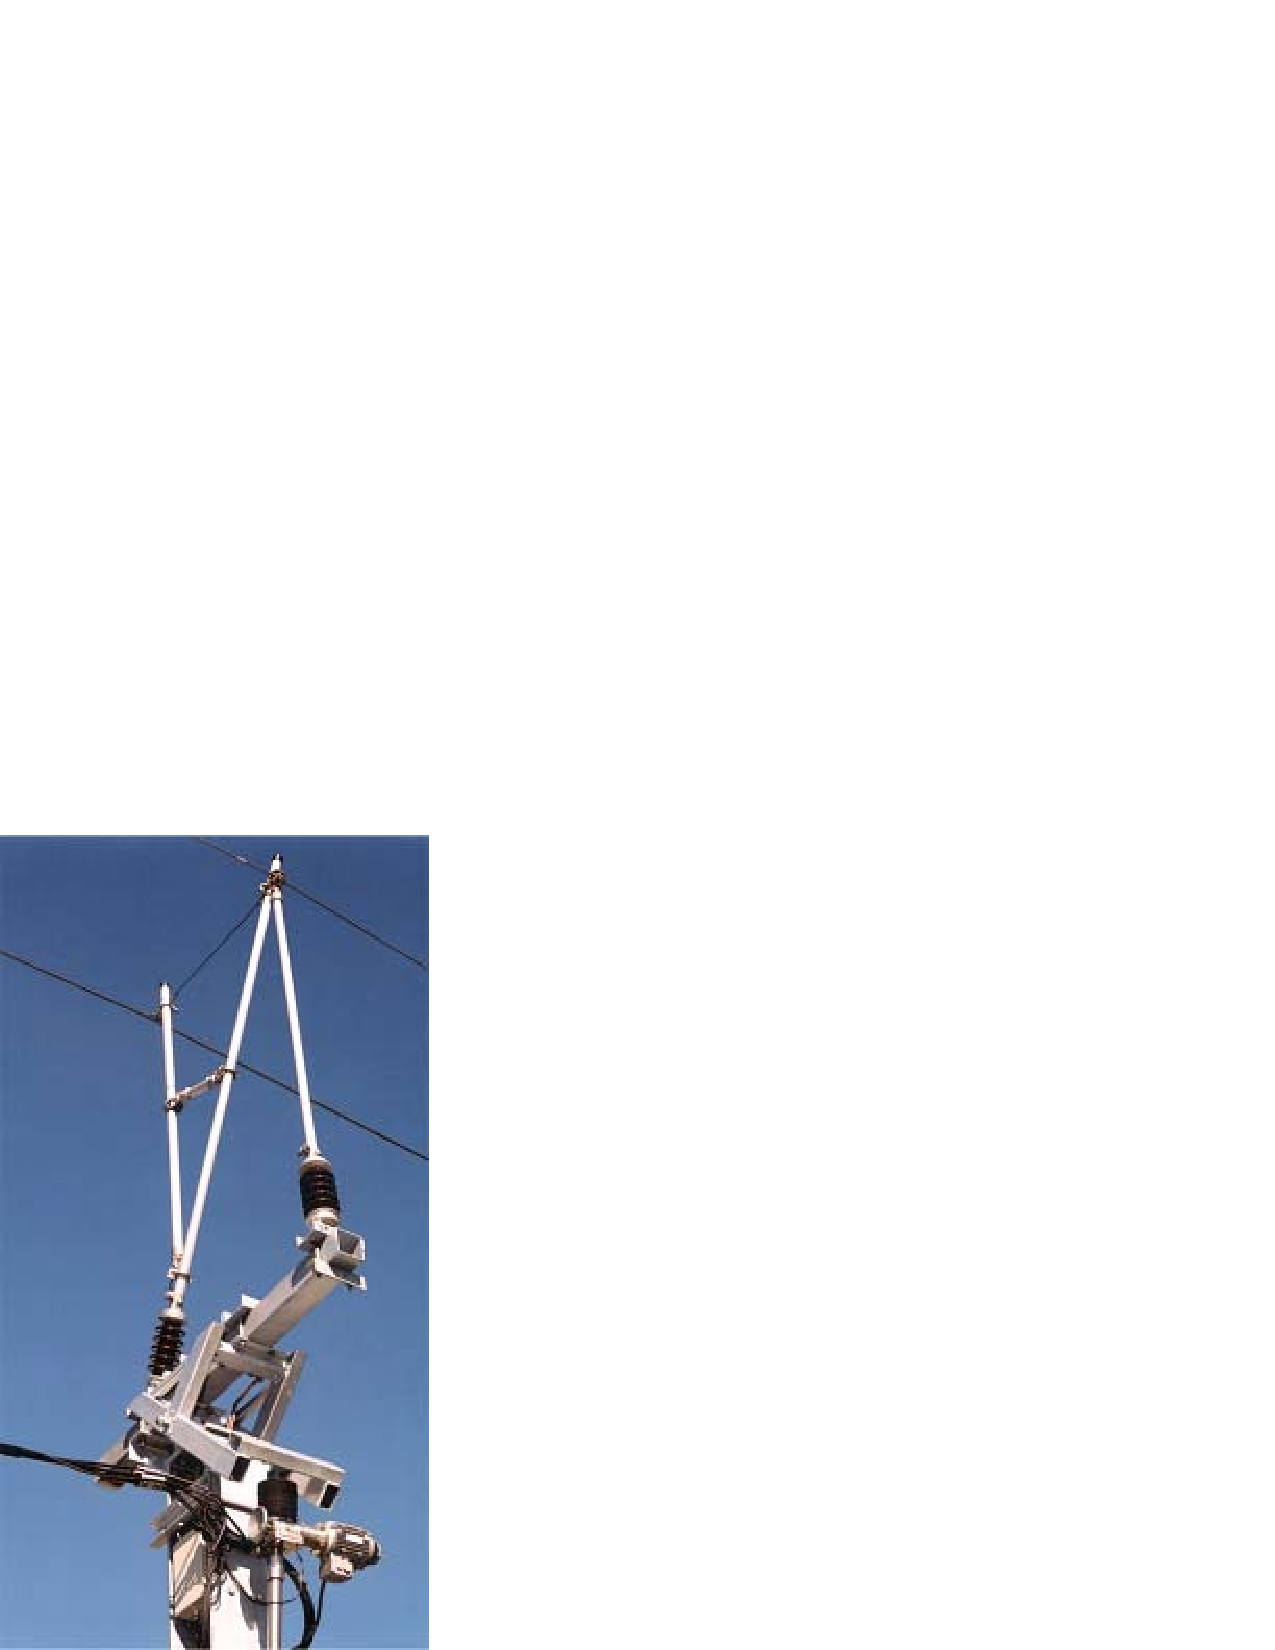
\includegraphics[width=4cm]{results/results_kfl_mast2}
%    \caption{Picture of the mast in up position}
%    \label{fig:results:kfl:mast2}
%\end{figure}


\subsubsection{Real Hardware}

Although this system is not mass-produced, there were nevertheless
cost constraints. Even a small FPGA is more expensive than a general
purpose CPU. To compensate for this, additional chips for the memory
and the FPGA configuration were optimized for cost. One standard
128KB Flash was used to hold FPGA configuration data, the Java
program and a logbook. External main memory was reduced to 128KB
with an 8-bit data bus.

To reduce external components, the boot process is a little
complicated. A watchdog circuit delivers a reset signal to a 32
macro-cell PLD. This PLD loads the configuration data into the FPGA.
When the FPGA starts, it disables the PLD and loads the Java program
from the Flash into the external RAM. After the JVM is initialized,
the program starts at \code{main()}.

The motor is controlled by silicon switches connected to the FPGA
with opto couplers. The position is measured with two end sensors and
a revolving sensor. The processor supervises the voltage and current
of the motor supply. A display and keyboard are attached to the base
station for the user interface. The communication bus (up to one
kilometer) is attached via an isolated RS485 data interface.

\subsubsection{Synthesized Hardware}

The following I/O modules were added to the JOP core in the FPGA:
%
\begin{itemize}
\item Timer
\item UART for debugging
\item UART with FIFO for the RS485 line
\item Four sigma delta ADCs
\item I/O ports
\end{itemize}
%
Five switches in the power line needed to be controlled by the
program. A wrong setting of the switches due to a software error
could result in a short circuit. Ensuring that this could not happen
was a straightforward task at the VHDL level. The sigma-delta ADCs
are used to measure the temperature of the silicon switches and the
current through the motor.

\subsubsection{Software Architecture}

The main task of the program was to measure the position using the
revolving sensor and communicate with the base station. This has to
be done under real-time constraints. This is not a very complicated
task. However, at the time of development, many features from a
full-blown JVM implementation, such as threads or objects, were
missing in JOP. The resulting Java was more like a \emph{tiny Java}.
It had to be kept in mind which Java constructs were supported by
JOP. Because there was no multi-threading capability, and in the
interests of simplicity, a simple infinite loop with constant time
intervals was used. Listing~\ref{lst:results:main} shows the
simplified program structure. After initialization and memory
allocation, this loop enters and never exits.

\begin{lstlisting}[float,caption=Simplified program structure,
label=lst:results:main]
    public static void main(String[] args) {

        init();
        Timer.start();
        forever();
        // this point is NEVER reached
    }

    private static void forever() {

        for (;;) {
            Msg.loop();
            Triac.loop();
            if (Msg.available) {
                handleMsg();
            } else {
                chkMsgTimeout();
            }
            handleWatchDog();
            Timer.waitForNextInterval();
        }
    }
\end{lstlisting}

\subsubsection{Communication}

Communication is based on a client-server structure. Only the base
station is allowed to send a request to a single mast station. The
station is then required to reply. The maximum reply time is bounded
by two time intervals. The base station handles timeout and retry. If
an irrecoverable error occurs, the base station switches off the
power to the mast stations, including the power supply to the motor.
This is the safe state of the whole system.

From the mast station perspective, every mast station supervises the
base station. The base station is required to send requests on a
regular basis. If this requirement is violated, the mast station
switches off its motor. The data is exchanged in small packets of
four bytes, including a one-byte CRC. To simplify the development,
commands to program the Flash in the mast stations and force a reset
were included. It is therefore possible to update the program, or
even change the FPGA configuration, over the network.

%\subsubsection{Benefits from using an FPGA}
%
%The flexibility of FPGAs made it possible to postpone some design
%decisions after production of the PCB. Since the production of the
%PBC was on the critical time line this helped to finish the complete
%project in time. During development, there have been situations
%where problems showed up that have not been foreseen.  Two examples
%are given where it was possible to find simple solutions:
%
%The routing of the PCB was almost finished. A question about cooling
%the switches (TRIAC) has arisen. The electronic development team
%insisted on a temperature sensor. The requirements in resolution and
%conversion time were low. A sigma-delta ADC with only two external
%passive components (a NTC thermistor and a capacitor) was
%implemented in the FPGA.
%
%When the sample rate for an ADC is low compared to the clock
%frequency of the digital system it is possible to transfer the AD
%conversion problem from the analogue to the time domain. In
%\figurename~\ref{fig_results_sigdel} the principle of a Sigma-Delta
%ADC is shown. Only the adder and the integrator have to be analogue
%components. A single bit DAC is just the FPGA digital output driving
%the signal between GND and VCCIO. The single bit ADC can be built
%with a comparator. For low resolution the threshold of the FPGA
%input is practical. The simplest form of an ADC built with an FPGA
%is shown in \figurename~\ref{fig_results_sigdel_real}. The filter
%averages $2^n$ samples and can be implemented as a counter.
%
%\begin{figure*}
%    \centering
%    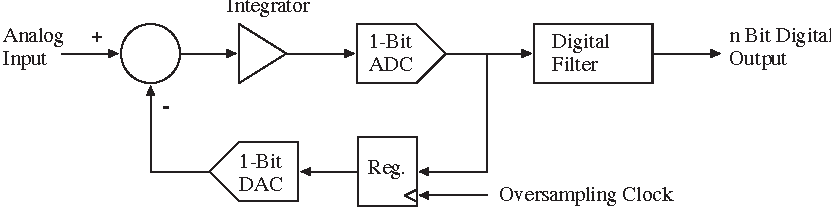
\includegraphics{results/results_sigdel}
%    \caption{A sigma-delta ADC}
%    \label{fig_results_sigdel}
%\end{figure*}
%
%
%\begin{figure*}
%    \centering
%    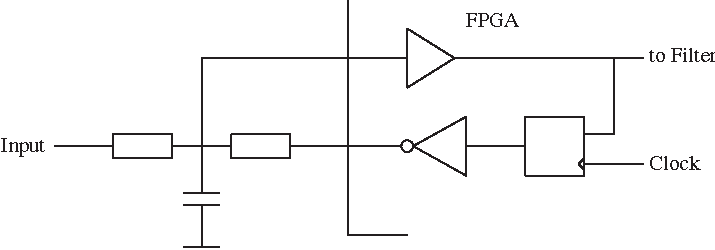
\includegraphics{results/results_sigdel_real}
%    \caption{A minimal sigma-delta ADC with an FPGA}
%    \label{fig_results_sigdel_real}
%\end{figure*}
%
%
%The AC current of the motor had to be monitored. The solution for
%this was a shunt resistor in every power line and an opto-coupler
%for isolation. However, it turned out that the shunt resistors got
%too hot and delivered to little voltage for the opto-couplers to
%work reliable. Having seen that it is possible to build an ADC in
%the FPGA a new idea was born. For EMC reasons, there is an inductor
%in every AC line. With a few windings of wire, a simple transformer
%can be built. The resulting voltage was amplified, rectified and
%used for current measurement. An additional comparator was used for
%an exacter threshold than the input buffer of the FPGA. This
%solution kept the board cool and added extra functionality. It is
%now possible to define two thresholds for too little and too much
%current.
%

\subsection{Further Projects}

TAL, short for TeleAlarm, is a remote tele-control and data logging
system. TAL communicates via a modem or an Ethernet bus with a SCADA
system or via SMS with a mobile phone. For this application, a
minimal TCP/IP stack needed to be implemented. This stack was the
reason for implementing threads and a simple real-time system in
JOP.

Another application of JOP is in a communication device with soft
real-time properties -- Austrian Railways' (\"OBB) new security
system for single-track lines. Each locomotive is equipped with a GPS
receiver and a communication device. The position of the train,
differential correction data for GPS, and commands are exchanged with
a server at the central station over a GPRS virtual private network.
JOP is the heart of the communication device in the locomotive. The
flexibility of the FPGA and an Internet connection to the embedded
system make it possible to upgrade the software and even the
processor in the field.


\section{Summary}

In this chapter, we presented an evaluation of JOP. We have seen
that JOP is the smallest hardware realization of the JVM available
to date. Due to the efficient implementation of the stack
architecture, JOP is also smaller than a \emph{comparable} RISC
processor in an FPGA. Implemented in an FPGA, JOP has the highest
clock frequency of all known Java processors.

We compared JOP against several embedded Java systems and, as a
reference, with Java on a standard PC. A Java processor is up to 500
times faster than an interpreting JVM on a standard processor for an
embedded system. JOP is about six times faster than the aJ80 Java
processor and as fast as the aJ100\footnote{The measured aJ100
system contained faster SRAMs than the FPGA board for JOP.}.
Preliminary results using compiled Java for a RISC processor in an
FPGA, with a similar resource usage and maximum clock frequency to
JOP, showed that native execution of Java bytecodes is faster than
compiled Java.

We compared the basic properties of the real-time scheduler on JOP
against the RTSJ implementation on Linux. The integration of the
scheduler in the JVM, and the timer interrupt under scheduler
control, results in an efficient platform for Java in embedded
real-time systems. JOP performs better and more predictably than the
reference implementation of the RTSJ under Linux.

We also performed WCET analysis of the implemented JVM at the
microcode level. This analysis provides the WCET and BCET values for
the individual bytecodes. We have also shown that there are no
dependencies between individual bytecodes. This feature, in
combination with the method cache (see Section~\ref{sec:cache}),
makes JOP an easy target for low-level WCET analysis of Java
applications.

Usage of JOP in three real-world applications showed that the
processor is mature enough to be used in commercial projects.


%\bibliographystyle{plain}
%\bibliography{../bib/mybib}
%\end{document}
